\documentclass[11pt,a4paper]{article}
			\usepackage[french]{babel}
					
				\usepackage{pifont}
				\usepackage{textcomp}
				\usepackage{makeidx}
				\usepackage{tabularx}
				\usepackage{multicol}
				\usepackage{multirow}
				\usepackage{longtable}
				\usepackage{color}
				\usepackage{soul}
				\usepackage{boxedminipage}
				\usepackage{shadow}
				\usepackage{framed}			
				\usepackage{array}
				\usepackage{url}
				\usepackage{ragged2e}
				\ifx\pdfoutput\undefined
					\usepackage{graphicx}
				\else
					\usepackage[pdftex]{graphicx}
				\fi
				\usepackage[a4paper, hyperfigures=true, colorlinks, linkcolor=black, citecolor=blue,urlcolor=blue, pagebackref=true, bookmarks=true, bookmarksopen=true,bookmarksnumbered=true,
                pdfauthor={}, pdftitle={TD1 - Prise en main de l’environnement}, pdfkeywords={TD1 - Prise en main de l'environnement, },pdfpagemode=UseOutlines,pdfpagetransition=Dissolve,nesting=true,
				backref, pdffitwindow=true, bookmarksnumbered=true]{hyperref}
				\usepackage{supertabular}
				\usepackage[table]{xcolor}
				\usepackage{url}
				\usepackage{caption} 
				\setlength{\parskip}{1.3ex plus 0.2ex minus 0.2ex}
				\setlength{\parindent}{0pt}
				
				\makeatletter
				\def\url@leostyle{ \@ifundefined{selectfont}{\def\UrlFont{\sf}}{\def\UrlFont{\footnotesize\ttfamily}}}
				\makeatother
				\urlstyle{leo}
				
				\definecolor{examplecolor}{rgb}{0.156,0.333,0.443}
				\definecolor{definitioncolor}{rgb}{0.709,0.784,0.454}
				\definecolor{exercisecolor}{rgb}{0.49,0.639,0}
				\definecolor{hintcolor}{rgb}{0.941,0.674,0.196}
				\definecolor{tableHeadercolor}{rgb}{0.709,0.784,0.454}
				\definecolor{tablerowAltcolor}{rgb}{.866,.905,.737}
				\definecolor{tablerowAlt2color}{rgb}{.968,.976,.933}
				
				\newenvironment{fshaded}{
				\def\FrameCommand{\fcolorbox{framecolor}{shadecolor}}
				\MakeFramed {\FrameRestore}}
				{\endMakeFramed}
				
				\newenvironment{fexample}[1][]{\definecolor{shadecolor}{rgb}{.913,.913,.913}
				\definecolor{framecolor}{rgb}{.156,.333,.443}
				\begin{fshaded}}{\end{fshaded}} 
				
				\newenvironment{fdefinition}{\definecolor{shadecolor}{rgb}{.913,.913,.913}
				\definecolor{framecolor}{rgb}{.709,.784,.454}
				\begin{fshaded}}{\end{fshaded}}
				
				\newenvironment{fexercise}{\definecolor{shadecolor}{rgb}{.913,.913,.913}
				\definecolor{framecolor}{rgb}{.49,.639,0}
				\begin{fshaded}}{\end{fshaded}}
				
				\newenvironment{fhint}{\definecolor{shadecolor}{rgb}{.913,.913,.913}
				\definecolor{framecolor}{rgb}{.941,.674,.196}
				\begin{fshaded}}{\end{fshaded}}	
				
				\newcommand{\PreserveBackslash}[1]{
				\let\temp=\\#1\let\\=\temp
				}
				\let\PBS=\PreserveBackslash
				\newcolumntype{A}{>{\PBS\raggedright\small\hspace{0pt}}X}
				\newcolumntype{L}[1]{>{\PBS\raggedright\small\hspace{0pt}}p{#1}}
				\newcolumntype{R}[1]{>{\PBS\raggedleft\small\hspace{0pt}}p{#1}}
				\newcolumntype{C}[1]{>{\PBS\centering\small\hspace{0pt}}p{#1}}
				
				\makeindex
				
				\title{TD1 - Prise en main de l'environnement}	
				\author{}
				\date{\today}
				
				\begin{document}
				
				\maketitle
				\clearpage
                {Table des mati\`eres}
                \tableofcontents
                
                \pagestyle{headings}
            
					\clearpage
				
			
		\section{TD1 - Prise en main de l'environnement} 
		\label{TD1index.tex}
			
			
		\subsection{TD1 - Prise en main de l'environnement} 
		\label{TD1unitTD1.tex}
			
			
		\subparagraph{Bravo !} 
		
					\textcolor{white}{.} \par
				
            \par
        
Si vous lisez cette page c'est que vous avez pu vous connecter sur  le PC.
Vous allez \`a pr\'esent voir comment l'utiliser correctement  pour les laboratoires Java.

			
		\subparagraph{Consignes} 
		
					\textcolor{white}{.} \par
				
            \par
        
Ces pages vont vous guider dans votre apprentissage de Java et Linux.

					\begin{enumerate}
				
			\item 
	Faites bien tous les exercices propos\'es;
			\item N'h\'esitez pas \`a  \textbf{montrer votre travail}  \`a votre professeur;
			\item N'h\'esitez pas \`a  \textbf{poser des questions}  si vous n'avez pas bien compris ce qu'on vous demande;
			\item  \textbf{Prenez des notes} ! Ce que vous allez apprendre aujourd'hui vous servira les semaines prochaines mais vous en aurez oubli\'e une grande partie si vous ne notez rien. Le plus pratique est probablement d'annoter la version  \textbf{papier} .
			\item Ayez toujours avec vous le  \textbf{guide visuel } et l' \textbf{aide-m\'emoire} . Ils vous seront utiles tout au long des tds.
					\end{enumerate}
				
			
		\subsubsection{Windows - Changer le mot de passe} 
		\label{TD1TD1learningObject1.tex}
			
			
		\subparagraph{Objectif} 
		
					\textcolor{white}{.} \par
				
            \par
        
Vous allez apprendre \`a modifier votre mot de passe.

			
		\subparagraph{R\'eflexion} 
		
					\textcolor{white}{.} \par
				
            \par
        
\`A votre avis, pourquoi vous demande-t-on de modifier votre mot de passe ?

			\begin{boxedminipage}[h]{\linewidth}
		Le mot de passe initial peut \^etre  \textit{trouv\'e } par un autre \'etudiant.
					\begin{enumerate}
				
			\item Celui qu'on vous a donn\'e n'est pas secret puisqu'il est not\'e dans un fichier informatique.
			\item il est tellement difficile \`a retenir que vous allez \^etre tent\'e de le noter quelque part.
					\end{enumerate}
				
Si un autre \'etudiant le connait, il peut se faire passer pour vous.

					\begin{enumerate}
				
			\item Les impressions qu'il fera vous seront factur\'ees.
			\item S'il commet un acte informatique ill\'egal, c'est vous qu'on soup\c connera \textit{} en premier. 
					\end{enumerate}
				
			\end{boxedminipage}

			
		\subparagraph{Exemples de mots de passe} 
		
                \textcolor{white}{.} \par
            
                    \textbf{\textit{
Quelles sont les propositions qui vous paraissent correctes comme mot de passe ? (plusieurs r\'eponses possibles)
}}
                
            \begin{itemize} 
        
            \item[ \ding{"6D} ] 
nadia

        
            \item[ \ding{"6D} ] 
m@C0p1ne

        
            \item[ \ding{"6D} ] 
GH5).jg

        
            \end{itemize} 
        
			
		\subparagraph{Changer le mot de passe} 
		
					\textcolor{white}{.} \par
				
            \par
        
Il est  temps de  \textbf{changer votre mot de passe} . Les \'etapes sont expliqu\'ees ici.
					\begin{enumerate}
				
			\item Appuyez sur ALT-CTRL-DEL  et choisissez Change password... . 
			\begin{boxedminipage}[h]{\linewidth}
		\begin{center}
					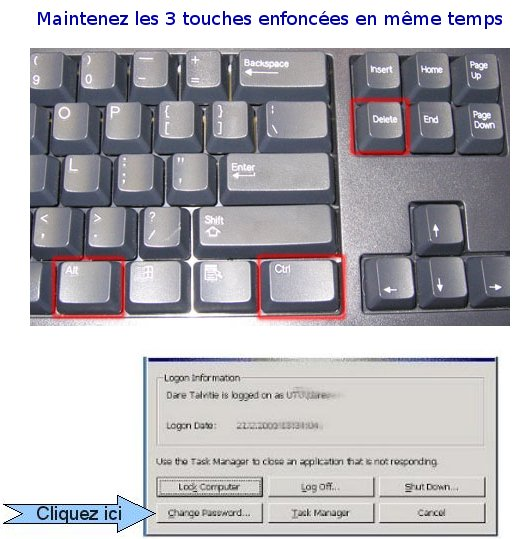
\includegraphics[width=0.8\linewidth,height=0.8\textheight,keepaspectratio=true]{/home/marco/Developpement/eLML8/LaboJava/TD1/fr/image/change_password_1.jpg}
						\end{center}
                
			\end{boxedminipage}

			\item Dans la fen\^etre qui apparait, tapez
	
					\begin{enumerate}
				
			\item votre mot de passe initial,
			\item le nouveau mot de passe,
			\item une deuxi\`eme fois ce nouveau mot de passe.
					\end{enumerate}
				 \textbf{Note}  : utilisez la souris ou la touche TAB  pour passer d'un champ \`a l'autre mais surtout pas la touche ENTER .
			\item Un message vous indique que tout s'est bien pass\'e (normalement).
	
					\begin{enumerate}
				
			\item Prenez le temps de le lire : c'est peut-\^etre un message d'erreur.
					\end{enumerate}
				 \textbf{Note}  : Prenez d'autant plus le temps si vous \'eprouvez des difficult\'es avec l'anglais; les messages d'erreurs seront g\'en\'eralement en anglais.  \textbf{Il faut absolument vous entrainer \`a lire des messages simples.} 
			\item Afin de v\'erifier que le mot de passe est bien chang\'e, d\'econnectez-vous et reconnectez-vous.
	(et revenez sur cette page bien s\^ur pour pouvoir continuer les exercices ;)) 
					\end{enumerate}
				 \textit{} 
			
		\subparagraph{FAQ} 
		
					\textcolor{white}{.} \par
				
            \par
         \textbf{Je ne suis pas content du mot de passe que j'ai choisi. Est-ce que je peux le changer ?} 
Oui mais pas tout de suite. L'administrateur des machines Windows de l'\'ecole impose un temps minimum (1 jour) entre 2 modifications de mot de passe.
 \textbf{Est-ce que je vais pouvoir garder ce mot de passe toute l'ann\'ee ?} 
Non. Pour des raisons de s\'ecurit\'e, Windows va vous demander de changer le mot de passe d'ici quelques mois.
 \textbf{J'ai oubli\'e mon mot de passe. Qu'est-ce que je peux faire ?} 
Les professeurs ne peuvent ni retrouver votre nouveau mot de passe, ni
remettre le mot de passe de d\'epart. Par contre le technicien (F.
Marchal qui a son bureau au 5\`eme) peut remettre le mot de passe de
d\'epart. Allez le trouver (et prenez garde \`a ce que \c ca n'arrive plus !)

			
		\subsubsection{Linux} 
		\label{TD1TD1learningObject2.tex}
			



\guillemotleft   \textit{Linux ? Il y a moins bien mais c'est plus cher}  \guillemotright . auteur inconnu 


  
			
		\subparagraph{Pr\'esentation} 
		
					\textcolor{white}{.} \par
				
            \par
        
Vous ne travaillerez pas directement sur votre PC durant les laboratoires Java.
Celui-ci vous servira pour vous connecter au serveur Linux (son nom est  \texttt{linux1} )
 \textbf{Tiens, c'est quoi Linux et pourquoi l'utiliser ? C'est quoi une machine partag\'ee?} 
Si vous vous posez encore ces questions, je vous invite vivement \`a relire le point 1 du guide visuel.
			
		\subsubsection{Se connecter} 
		\label{TD1TD1learningObject3.tex}
			

Lorsque vous allez vous connecter,  \texttt{linux1}  va vous demander de vous identifier.

					\begin{enumerate}
				
			\item Votre  \textbf{ \textit{username} }  est le m\^eme que sous Windows (avec un  \textbf{'g' minuscule}  obligatoirement).  \textbf{Note}  : pour Linux, les minuscules et les majuscules sont toujours des caract\`eres diff\'erents.Ex:  \texttt{g32010} 
			\item Votre  \textit{ \textbf{mot de passe} }  est le m\^eme que votre  \textbf{mot de passe initial sous Windows} .
					\end{enumerate}
				
  

Le mot de passe sous Windows et sous Linux sont 2 mots de passe
diff\'erents (initialis\'es \`a la m\^eme valeur). Vous avez modifi\'e votre mot
de passe sous Windows mais pas encore sous Linux (vous le ferez plus
tard...)

  
			
		\subparagraph{Connectez-vous \`a linux1} 
		
					\textcolor{white}{.} \par
				
            \par
        
Il y a 3 \'etapes:

					\begin{enumerate}
				
			\item Lancez l'application  \texttt{putty}  (vous la trouverez dans le menu ou comme raccourci sur le bureau).
	
			\item Indiquez \`a putty le nom de la machine ( \textit{Host Name} ) \`a laquelle vous voulez vous connecter (ici  \texttt{linux1} ). 
			\begin{boxedminipage}[h]{\linewidth}
		\begin{center}
					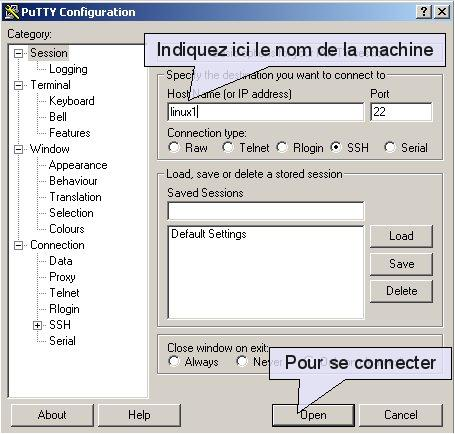
\includegraphics[width=0.8\linewidth,height=0.8\textheight,keepaspectratio=true]{/home/marco/Developpement/eLML8/LaboJava/TD1/fr/image/putty-login.jpg}
						\end{center}
                
			\end{boxedminipage}

			\item Cliquez sur '' \textbf{Open} ''; la connexion se fait ! S'il vous pr\'esente une boite de message avec un '' \textbf{Security Alert} '', cliquez sur '' \textbf{Yes} '' en toute confiance.
	
			\item Identifiez-vous !
	
					\begin{enumerate}
				
			\item Tapez votre nom d'utilisateur (gxxxxx ) puis sur la touche ENTREE . \textbf{Note } : Le clavier num\'erique ne fonctionne pas encore; nous verrons comment le configurer.
					\end{enumerate}
				
					\begin{enumerate}
				
			\item Tapez votre mot de passe puis sur la touche ENTREE .  \textbf{Note } : Rien ne s'affiche quand vous tapez votre mot de passe; c'est normal. 
					\end{enumerate}
				
					\end{enumerate}
				
			
		\subsubsection{Le mode console} 
		\label{TD1TD1learningObject4.tex}
			

Si vous ne savez plus ce qu'est le mode console ou comment entrer une commande, retournez d'abord faire un petit tour aux points 2 et 3 du guide visuel.

  
			
		\subparagraph{Ma premi\`ere commande} 
		
					\textcolor{white}{.} \par
				
            \par
        
Entrez la commande ls  (n'oubliez pas la touche ENTREE ).

Vous constatez que le bash a affich\'e quelque chose (d'incompr\'ehensible
pour le moment; ne vous inqui\'etez pas nous y reviendrons) et qu'il vous propose \`a nouveau l'invite de commande. 

			
		\subparagraph{Il faut \^etre pr\'ecis !} 
		
					\textcolor{white}{.} \par
				
            \par
        
Entrez \`a pr\'esent  la commande LS .

Vous voyez que le r\'esultat est diff\'erent : il ne comprend pas ce que vous lui voulez. En Linux,  \textbf{les majuscules et les minuscules n'ont pas le m\^eme sens, vous devez respecter la casse.} 
Faites une autre exp\'erience. Tapez les 3 commandes suivantes qui ne se diff\'erencient que par la pr\'esence ou non d'espaces. 

					\begin{enumerate}
				
			\item ls /home 
			\item ls/home 
			\item ls / home 
					\end{enumerate}
				
\`A nouveau le r\'esultat est diff\'erent dans les 3 cas.  \textbf{Les espaces ont de l'importance} .






Entrez \`a pr\'esent  la commande LS .

Vous voyez que le r\'esultat est diff\'erent : il ne comprend pas ce que vous lui voulez. En Linux,  \textbf{les majuscules et les minuscules n'ont pas le m\^eme sens, vous devez respecter la casse.} 
Faites une autre exp\'erience. Tapez les 3 commandes suivantes qui ne se diff\'erencient que par la pr\'esence ou non d'espaces. 

					\begin{enumerate}
				
			\item ls /home 
			\item ls/home 
			\item ls / home 
					\end{enumerate}
				
\`A nouveau le r\'esultat est diff\'erent dans les 3 cas.  \textbf{Les espaces ont de l'importance} .



			
		\subsubsection{Changer le mot de passe} 
		\label{TD1TD1learningObject5.tex}
			
La commande pour changer le mot de passe est passwd .

					\begin{enumerate}
				
			\item Les r\`egles \`a respecter sont quasiment les m\^emes que sur Windows. Attention toutefois \`a ne pas choisir un mot du dictionnaire.
			\item Vous pouvez d'ailleurs reprendre le m\^eme mot de passe que celui que vous avez choisi pour Windows. 
					\end{enumerate}
				
			
		\subparagraph{\`A vous !} 
		
					\textcolor{white}{.} \par
				
            \par
        
Tapez la commande ad\'equate pour changer votre mot de passe.

					\begin{enumerate}
				
			\item Le syst\`eme vous demande de taper le mot de passe actuel (vous ne le voyez pas quand vous le tapez, c'est normal !)
			\item Ensuite, vous entrez le nouveau mot de passe que vous venez de choisir.
			\item Vous retapez une deuxi\`eme fois ce mot de passe pour le confirmer.
					\end{enumerate}
				 \textbf{Si \c ca va mal...} 
					\begin{enumerate}
				
			\item  \textit{Quand je tape la commande rien ne se passe !} 
					\begin{enumerate}
				
			\item Avez-vous bien appuy\'e sur la touche ENTREE  ?
			\item Une seule personne \`a la fois peut changer son mot de passe. Soyez patient.
					\end{enumerate}
				
			\item  \textit{Apr\`es avoir tout entr\'e, il me met un message d'erreur !} 
					\begin{enumerate}
				
			\item  \textbf{Lisez le message}  ! Il est en g\'en\'eral assez explicite.
			\item Peut-\^etre que le mot de passe est trop simple.
			\item Peut-\^etre n'avez-vous pas respect\'e les minuscules/majuscules.
					\end{enumerate}
				
					\end{enumerate}
				
			
		\subparagraph{V\'erification} 
		
					\textcolor{white}{.} \par
				
            \par
        
Pour v\'erifier que tout s'est bien pass\'e, vous pouvez vous d\'econnecter et vous reconnecter. Pour quitter proprement  \texttt{linux1} , la commande est exit .

			
		\subparagraph{FAQ} 
		
					\textcolor{white}{.} \par
				
            \par
         \textbf{Vous me dites que la commande pour changer le mot de passe est passwd  et que celle pour quitter est exit . Je vais devoir retenir tout \c ca ?} 
Oui ! En tout cas pour les plus fr\'equentes mais l'apprentissage se fera naturellement \`a force de les utiliser.
 \textbf{Et si j'ai oubli\'e le nom d'une commande ?} 
Vous verrez la semaine prochaine les moyens \`a votre disposition pour retrouver le nom d'une commande ou comment l'utiliser correctement. 

			
		\subparagraph{FAQ} 
		
					\textcolor{white}{.} \par
				
            \par
         \textbf{J'ai quitt\'e en fermant la fen\^etre, c'est pas plus simple ?} 
Oui ! Mais c'est impoli de quitter quelqu'un sans lui dire au revoir !
;) Plus s\'erieusement, vous coupez brutalement la conversation avec
 \texttt{linux1}  ce qui peut laisser trainer des programmes actifs et vous emp\^echer de
vous connecter la prochaine fois.
 \textbf{J'ai oubli\'e mon mot de passe. Je dois aussi aller voir F. Marchal ?} 
Non ! Votre professeur de Java peut r\'einitialiser le mot de passe Linux \`a sa valeur initiale.

			
		\subsubsection{Le dossier personnel et le dossier courant} 
		\label{TD1TD1learningObject6.tex}
			
Un petit tour pr\'ealable aux points 4 \`a 7 du guide visuel est vivement conseill\'e.

			
		\subparagraph{Examiner son dossier} 
		
					\textcolor{white}{.} \par
				
            \par
        
Comment voir le contenu de votre dossier ? Simplement avec la commande ls  que vous avez d\'ej\`a rencontr\'ee.

			
		\subparagraph{Exp\'erimentation} 
		
					\textcolor{white}{.} \par
				
            \par
        
Tapez la commande ls 
					\begin{enumerate}
				
			\item Il vous montre le contenu de votre dossier.
			\item Vous constatez qu'il contient d\'ej\`a des \'el\'ements.
			\item La couleur permet de distinguer un dossier (en bleu) d'un fichier (en blanc).
			\item Comme
	sur Windows, la notion de dossier est hi\'erarchique : un dossier peut
	contenir des fichiers mais aussi d'autres dossiers qui \`a leur tour...
					\end{enumerate}
				
Tapez la commande ls bin .

					\begin{enumerate}
				
			\item Cette fois, il vous montre le contenu du dossier  \textit{bin}  (ne vous inqui\'etez pas, la commande n'affiche rien parce que le dossier est vide).
					\end{enumerate}
				
\`A pr\'esent, tapez la commande cd bin .

					\begin{enumerate}
				
			\item Cette commande demande de se  \textit{ \textbf{d\'eplacer} }  dans le dossier  \textit{bin} .
					\end{enumerate}
				
Retapez la commande ls  du d\'ebut.

					\begin{enumerate}
				
			\item Le r\'esultat est diff\'erent. Est-ce que vous comprenez pourquoi ?
					\end{enumerate}
				
			
		\subparagraph{Le dossier courant} 
		
					\textcolor{white}{.} \par
				
            \par
        
\`A tout moment, vous \^etes  \textit{dans}  un dossier, appel\'e le  \textbf{dossier courant}  ( \textit{working directory}  en anglais).

					\begin{enumerate}
				
			\item La commande cd  ( \textit{change directory} ) permet de changer de dossier courant.
			\item La commande pwd  ( \textit{print working directory)}  permet d'afficher le chemin du dossier courant (o\`u vous \^etes pour le moment).
					\end{enumerate}
				 \textbf{C'est quoi le chemin ?}  C'est la suite des dossiers qu'il faut traverser. Nous verrons \c ca plus en d\'etail dans le prochain TD. 

			
		\subparagraph{Exp\'erimentation} 
		
					\textcolor{white}{.} \par
				
            \par
        
					\begin{enumerate}
				
			\item 
	En pr\'eambule, tapez la commande cd  pour revenir dans votre  \textit{home}  (dossier personnel).
			\item Tapez \`a pr\'esent la commande ls bin .
			\item Comparez le r\'esultat avec celui produit par les 2 commandes suivantes : cd bin  et ls 
					\end{enumerate}
				
			
		\subparagraph{Question} 
		
					\textcolor{white}{.} \par
				
            \par
        
Est-ce qu'on peut dire que
ls bin 
est strictement \'equivalent \`a
cd bin ls 
?

Comment le mettre en \'evidence ?

			\begin{boxedminipage}[h]{\linewidth}
		
Non ! Dans le 1er cas, on ne modifie pas le dossier courant. Dans le 2\`eme cas oui. On peut le mettre en \'evidence en tapant la commande pwd  apr\`es chaque cas.

			\end{boxedminipage}

			
		\subsubsection{L'\'editeur} 
		\label{TD1TD1learningObject7.tex}
			

Un petit tour pr\'ealable au point 8 du guide visuel est vivement conseill\'e.

  
			
		\subparagraph{Exp\'erimentation} 
		
					\textcolor{white}{.} \par
				
            \par
        
					\begin{enumerate}
				
			\item En pr\'eambule, tapez la commande cd  pour revenir dans votre  \textit{home}  (dossier personnel).
	
			\item Tapez vi test  pour commencer \`a \'editer le fichier  \texttt{test}  (comme il n'existe pas encore, il est cr\'e\'e).
			\item Pour le moment, vous \^etes en mode  \textit{commande} . Tapez i  pour entrer en mode  \textit{insertion}  (constatez le changement en bas de la fen\^etre). 
			\item Entrez quelques mots puis appuyez sur la touche ESC  pour revenir au mode  \textit{commande} .
			\item Tapez :  pour entrer en mode  \textit{ex\'ecution}  et entrez x  suivi de enter  (votre travail est sauv\'e et vous sortez de l'\'editeur). 
			\item Tapez \`a pr\'esent la commande ls . Vous pouvez constater que le fichier  \texttt{test}  est apparu dans la liste ;)
					\end{enumerate}
				 \textbf{Note}  : si vous \^etes en mode  \textit{commande}  et que vous voulez effacer un caract\`ere, essayez x .

Il existe bien s\^ur encore beaucoup de choses \`a apprendre sur cet \'editeur mais c'est d\'ej\`a bien pour un d\'ebut; nous y reviendrons un peu plus tard.
			
		\subsubsection{Quelques commandes courantes} 
		\label{TD1TD1learningObject8.tex}
			
			
		\subparagraph{Faisons le point} 
		
                \textcolor{white}{.} \par
            
Vous avez d\'ej\`a eu l'occasion d'utiliser 6 commandes : passwd , ls , cd , pwd , exit  et vi . Voyons voir si vous avez retenu leur signification.

					\begin{enumerate}
				
			\item La commande pour voir le contenu d'un dossier (la liste de ce qu'il contient) est    
  \_\_\_\_\_\_\_\_\_\_\_ 
			\item La commande pour \'editer le contenu d'un fichier est    
  \_\_\_\_\_\_\_\_\_\_\_ 
			\item La commande pour changer son mot de passe est   
  \_\_\_\_\_\_\_\_\_\_\_ 
			\item La commande pour se d\'econnecter de linux1 est   
  \_\_\_\_\_\_\_\_\_\_\_ 
			\item La commande pour changer de dossier courant est         
  \_\_\_\_\_\_\_\_\_\_\_ 
			\item La commande pour voir le chemin du dossier courant est    
  \_\_\_\_\_\_\_\_\_\_\_ 
					\end{enumerate}
				
			
		\subparagraph{Quelques commandes en plus...} 
		
					\textcolor{white}{.} \par
				
            \par
        
Il est temps de voir quelques commandes suppl\'ementaires.

					\begin{enumerate}
				
			\item cat nomDuFichier  affiche \`a l'\'ecran le contenu du fichier dont le nom est donn\'e (ce n'est pas un \'editeur, on voit le contenu et c'est tout);
			\item mkdir nomDuDossier  cr\'ee un dossier (vide);
			\item mv nomDuFichier nouveauNomDeFichier  renomme le fichier donn\'e sous le nom ''nouveauNomDeFichier'';
			\item mv nomDuFichier nomDuDossier  d\'eplace le fichier donn\'e dans le dossier indiqu\'e; 
			\item cp nomDuFichier nouveauNomDeFichier  cr\'ee une copie du fichier sous le nom ''nouveauNomDeFichier'';
			\item mv nomDuFichier nomDuDossier  copie le fichier donn\'e dans le dossier indiqu\'e;
			\item rm fichier  d\'etruit le fichier dont on donne le nom; 
			\item rmdir dossier  d\'etruit le dossier dont on donne le nom (Attention, le dossier doit \^etre vide !). 
					\end{enumerate}
				
			
		\subparagraph{Exercice 1} 
		
					\textcolor{white}{.} \par
				
            \par
        
Cr\'eez un dossier  \texttt{td1}  et d\'eplacez-y le fichier de test que vous avez d\'ej\`a cr\'e\'e.
 \textbf{Rappel}  : Notez bien votre r\'eponse. Il est difficile de tout retenir la premi\`ere fois; vous serez bien content la semaine prochaine de pouvoir retrouver comment vous avez fait !

			
		\subparagraph{Exercice 2} 
		
					\textcolor{white}{.} \par
				
            \par
        
					\begin{enumerate}
				
			\item 
	Prenez une copie de votre fichier de test (appelez-la  \texttt{test2} ). 
			\item \'Editez ce fichier et ajoutez-y quelques mots. 
			\item Affichez le contenu des 2 fichiers pour v\'erifier qu'ils sont bien diff\'erents.
	
					\end{enumerate}
				
			
		\subparagraph{Exercice 3} 
		
					\textcolor{white}{.} \par
				
            \par
        
					\begin{enumerate}
				
			\item 
	Cr\'eez, dans votre dossier  \texttt{td1} , un dossier  \texttt{monDossier} . 
			\item D\'eplacez-y votre fichier  \texttt{test2} .
					\end{enumerate}
				
			
		\subparagraph{Exercice 4} 
		
					\textcolor{white}{.} \par
				
            \par
        
D\'etruisez le dossier  \texttt{monDossier}  (ainsi que son contenu).

			
		\subsubsection{L'\'editeur (le retour)} 
		\label{TD1TD1learningObject9.tex}
			
Revenons sur l'\'editeur et apprenons quelques commandes suppl\'ementaires

					\begin{enumerate}
				
			\item :w  permet de  \textit{sauver sans quitter}  l'\'editeur; 
			\item :w nom  permet de  \textit{sauver sous le nom donn\'e} ;
			\item :q!  permet de  \textit{quitter}  l'\'editeur  \textit{sans sauver} ;
			\item x  \textit{efface un caract\`ere} ;
			\item dd  \textit{coupe}  la ligne sous le curseur;
			\item yy  \textit{copie}  la ligne sous le curseur;
			\item p  \textit{colle}  la ligne pr\'ec\'edemment copi\'ee ou coup\'ee.
					\end{enumerate}
				
			
		\subparagraph{Exercice} 
		
					\textcolor{white}{.} \par
				
            \par
        
Mettons tout \c ca en pratique au travers d'un petit exercice. Nous avons cr\'e\'e sur  \texttt{linux1}  un petit fichier (son nom est  \texttt{/eCours/java/td/td1/notes} ). Votre objectif est de le copier chez vous (dans votre dossier  \texttt{td1} ) et d'y apporter quelques modifications. 

					\begin{enumerate}
				
			\item R\'eorganisez les lignes pour qu'elles soient dans l'ordre.
			\item Remplacez l'acronyme par votre login et la date par la date du jour.
					\end{enumerate}
				
			
		\subsubsection{Conclusion} 
		\label{TD1TD1learningObject10.tex}
			
			
		\subparagraph{Bravo} 
		
					\textcolor{white}{.} \par
				
            \par
        
Vous \^etes arriv\'es au bout de ce premier TD. Avant de quitter le laboratoire, n'oubliez pas de :

					\begin{enumerate}
				
			\item quitter proprement la connexion avec  \texttt{linux1}  (exit ).
			\item \'eteindre l'ordinateur.
					\end{enumerate}
				
Attention, afin d'arriver au laboratoire dans les meilleures conditions, il est 
bien de revoir la mati\`ere qui sera mise en pratique. C'est pourquoi nous
vous fournissons quelques exercices pr\'eparatoires \`a faire \`a la maison 
pour vous permettre d'\'evaluer si vous \^etes pr\^et. Afin de v\'erifier que vous pr\'eparez bien ces exercices, une interrogation sera faite avant de d\'emarrer chaque labo.

\`A la semaine prochaine et soyez \`a l'heure !

			
		\subparagraph{Ressources} 
		
					\textcolor{white}{.} \par
				
            \par
        
Vous voulez en savoir plus sur ce que vous avez fait aujourd'hui ?

Nous avons rassembl\'e sur le site ( \textbf{suivez le lien ''Aide''} ), une s\'erie de documents qui peuvent \^etre utiles. Voyez notamment :  

					\begin{enumerate}
				
			\item Un  \textbf{guide visuel Linux} que vous avez d\'ej\`a utilis\'e;
			\item Un  \textbf{aide-m\'emoire}  \'ecrit par nos soins sur l'utilisation de Windows et Linux; 
			\item Un  \textbf{quick reference}  sur l'utilisation de  \textbf{vi} ; 
			\item Un  \textbf{quick reference}  sur les commandes  \textbf{linux} . 
					\end{enumerate}
				
				\end{document}
			